\subsubsection{Общая структура програмной компоненты}

\begin{figure}[ht!]
    \centering
    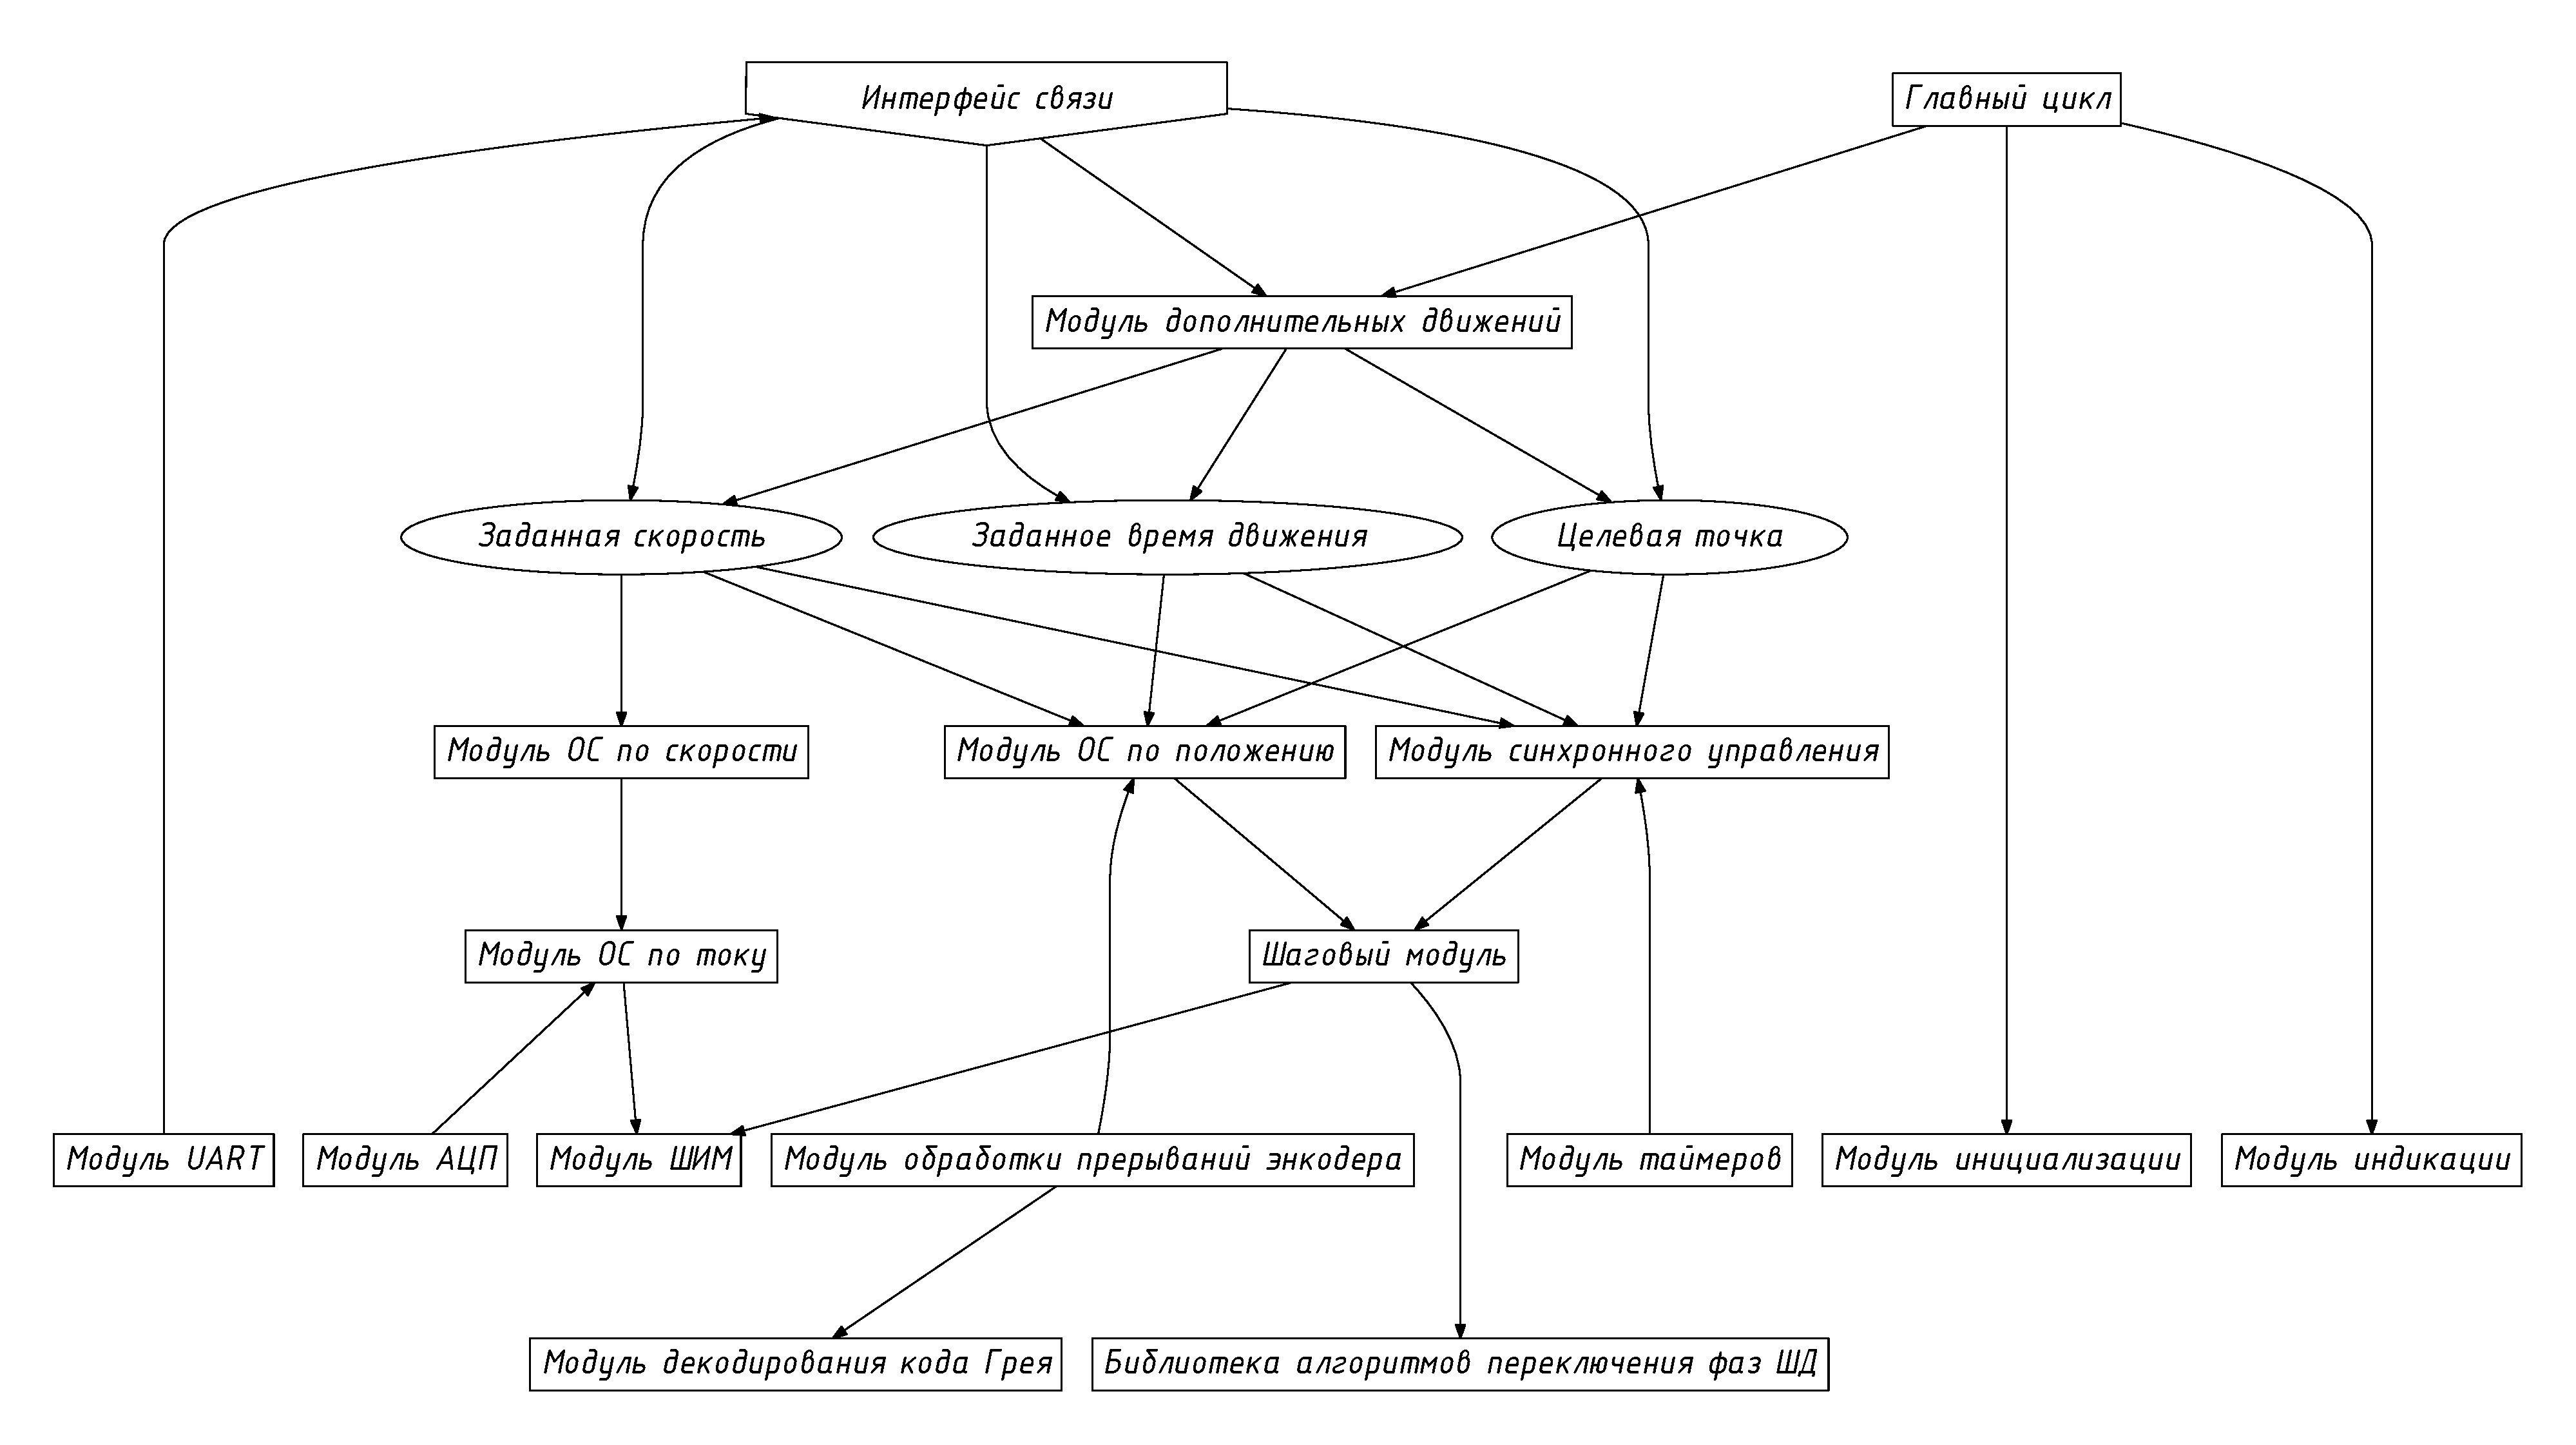
\includegraphics[width=1.2\linewidth, angle=90, keepaspectratio]
                    {src/pictures/soft_arch.pdf}
    \caption{Архитектура програмной компоненты}
    \label{control_object_general_view}
\end{figure}

\subsubsection{Шаговый модуль}
Шаговый модуль является интерфейсом переключения фаз шагового двигателя и
обладает только одним доступным другим модулям методом - методом включения
следующего (или предыдущего, в зависимости от желаемого направления движения)
алгоритмического шага управления двигателем (см. \ref{sec_step_control_algos}
о циклической природе алгоритмических шагов), фактически управляя только
полярностью напряжения, подаваемого на фазы.

Интерфейс модуля:
\begin{lstlisting}
void stop();
void nextStep();
void prevStep();
\end{lstlisting}

Модуль может работать в одном из трёх
алгоритмов переключения обмоток~--- однофазном, двухфазном или полуфазном.

Такая структура позволяет полностью изолировать более высокоуровневые модули от
того, как реализуются шаги двигателя, какой алгоритм переключения фаз
используется и т.д., оставляя при этом другим модулям ответственность о таких вещах
как поддержание требуемых токов и т.п.

\subsubsection{Модуль ОС по положению}
Для контура обратной связи по положению был споектирован модуль:
раздел \ref{module_control_modules_feedback_control},
стр. \pageref{module_control_modules_feedback_control}.

Обозначив направление движения как $\textit{dir} = \pm 1$ и объединив формулы
для двух направлений движений, получим из (\ref{movement_zone_posit_dir_for_delta})
и (\ref{movement_zone_negat_dir_for_delta}) для зоны движения

\begin{equation}
    \label{movement_zone_for_delta}
    \theta_\textit{ком} - \theta_\textit{шаг}
    < dir \cdot (\phi_\textit{акт} - \theta)
    \leq \theta_\textit{ком}
\end{equation}

и из (\ref{switch_zone_posit_dir_for_delta})
и (\ref{switch_zone_negat_dir_for_delta}) для зоны переключения

\begin{equation}
    \label{switch_zone_for_delta}
    \theta_\textit{ком} - 2\theta_\textit{шаг}
    < dir \cdot (\phi_\textit{акт} - \theta)
    \leq \theta_\textit{ком} - \theta_\textit{шаг}
\end{equation}

\paragraph{Зона выпада из синхронизма}
При попадании в зону выпада из синхронизма, не зависимо от причин приведших к этому,
модуль обратной связи по положению должен восстановить информацию о том,
в зоне переключения какой фазы ротор находится в данный момент. Полагаем, что для
продолжения движения в нужном направлении, необходимо, чтобы шаговый модуль
шаг в нужном направлении. Для этого необходимо обновить информацию о том, на каком
алгоритмическом шаге ротор двигателя находится в данный момент
(см. \ref{sec_step_control_algos} о циклической природе алгоритмических шагов).

Полагаем, что ротор находится в зоне переключения некоторой <<мнимо~--~активной>> фазы,
тогда информация об угловом положении вектора магнитного поля, которое бы имело место,
если бы фаза была действительно включена, позволит обновить информацию о текущем
алгоритмическом шаге шагового модуля. Это позволит шаговому модулю при получении
команды движения в заданном направлении запитать нужную фазу, сделав корректный
алгоритмический шаг.

Определеним формулы для вычисления углового вектора магнитного положения
<<мнимо~--~активной>> фазы для разных направлений движения.

\subparagraph{Положительное направление движения}

Из формулы (\ref{switch_zone_posit_dir_for_curr_pos}) получим

\begin{equation}
    \label{sync_restore_posit_dir_active_pole_pos_conditions}
    \phi_\textit{акт}
    \leq \theta + \theta_\textit{ком} - \theta_\textit{шаг}
    < \phi_\textit{акт} + \theta_\textit{шаг}
\end{equation}

Пусть $T = \theta + \theta_\textit{ком} - \theta_\textit{шаг}$, тогда

\begin{equation}
    \label{sync_restore_posit_dir_active_pole_pos}
    \phi_\textit{акт} = T - mod(T, \theta_\textit{шаг})
\end{equation}
где $mod$ - операция вычисления остатка от деления с сохранением знака делимого.

\subparagraph{Отрицательное направление движения}
Из формулы (\ref{switch_zone_negat_dir_for_curr_pos}) получим

\begin{equation}
    \label{sync_restore_negat_dir_active_pole_pos_conditions}
    \phi_\textit{акт} - \theta_\textit{шаг}
    < \theta - \theta_\textit{ком} + \theta_\textit{шаг}
    \leq \phi_\textit{акт}
\end{equation}

Пусть $D = \theta - \theta_\textit{ком} + \theta_\textit{шаг}$, тогда

\begin{equation}
    \label{sync_restore_negat_dir_active_pole_pos}
    \phi_\textit{акт} =
        \begin{cases}
            D,                                                      & \mbox{если } mod(D, \theta_\textit{шаг}) = 0 \\
            D - mod(D, \theta_\textit{шаг}) + \theta_\textit{шаг},  & \mbox{если } mod(D, \theta_\textit{шаг}) \ne 0)
        \end{cases}
\end{equation}
где $mod$ - операция вычисления остатка от деления с сохранением знака делимого.

\subsubsection{Скоростной модуль}
\subsubsection{Токовый модуль}
